\chapter{CodeBlue System Architecture}
\label{chap-codeblue}




\label{sec-cb-arch}


\section{Goals}
\label{sec-cb-goals}


In this chapter, we describe the design and implementation of CodeBlue, a
system architecture we propose for medical sensor networks.
Before describing the architecture, we first outline the core goals of
the CodeBlue platform. The requirements for medical sensor networks 
depend greatly on the specific application and deployment environment. 
For example, use of wireless sensors in specialized clinical settings
may not require all of the features described below. However, CodeBlue is
intended
to support a wide range of application requirements.


\begin{itemize}
\item {\bf Scalability and robustness:} 
CodeBlue should scale up to a large 
number of sensors and receiving devices. Hospital deployments may
involve thousands of individual sensors, often with multiple sensors
per patient. Hundreds of hospital staff may use handheld devices to
receive data from the network. Moreover, performance should degrade
gracefully as network load increases; for example, the network should 
avoid unfairly dropping data from a particular set of patients. 

\item
{\bf Multiple concurrent queries:} Doctors, nurses, and medics using
the CodeBlue system may issue queries specifying periodic or triggered
vital sign reports from differing, possibly overlapping sets of
patients. The system should efficiently handle multiple queries with
varying parameters.

\item
{\bf Ad-hoc deployment:} In emergency and disaster-response settings,
it is critical that the CodeBlue network be deployed rapidly, in an
{\em ad-hoc} fashion, without the use of a fixed network
infrastructure.  When powered on, devices should rapidly join the
network and establish communication routes as needed. Even in hospital
settings where fixed infrastructure may be in place, {\em ad-hoc}
routing can increase robustness and extend range to areas without
access point coverage.  Moreover, the network should support a
dynamically shifting population of sensor and end-user devices.

\item
{\bf Support a broad class of medical sensors:} New medical sensors
should be easily integrated with the running system.  These sensors
may involve multiple distinct channels, variable data rates, often
ranging from less than 1~Hz to 1000~Hz, and specialized data
processing (e.g., an algorithm to detect tachycardia from blood oxygen
levels).


\item
{\bf External programmatic interface:} To support a wide range of
applications, CodeBlue should not be designed as a ``closed system''
using only specialized protocols for sensor querying and data
acquisition. A rich external interface, using industry-standard
protocols, greatly facilitates application integration.

\end{itemize}

\section{CodeBlue Architecture}

\begin{figure}[t]
\begin{center}
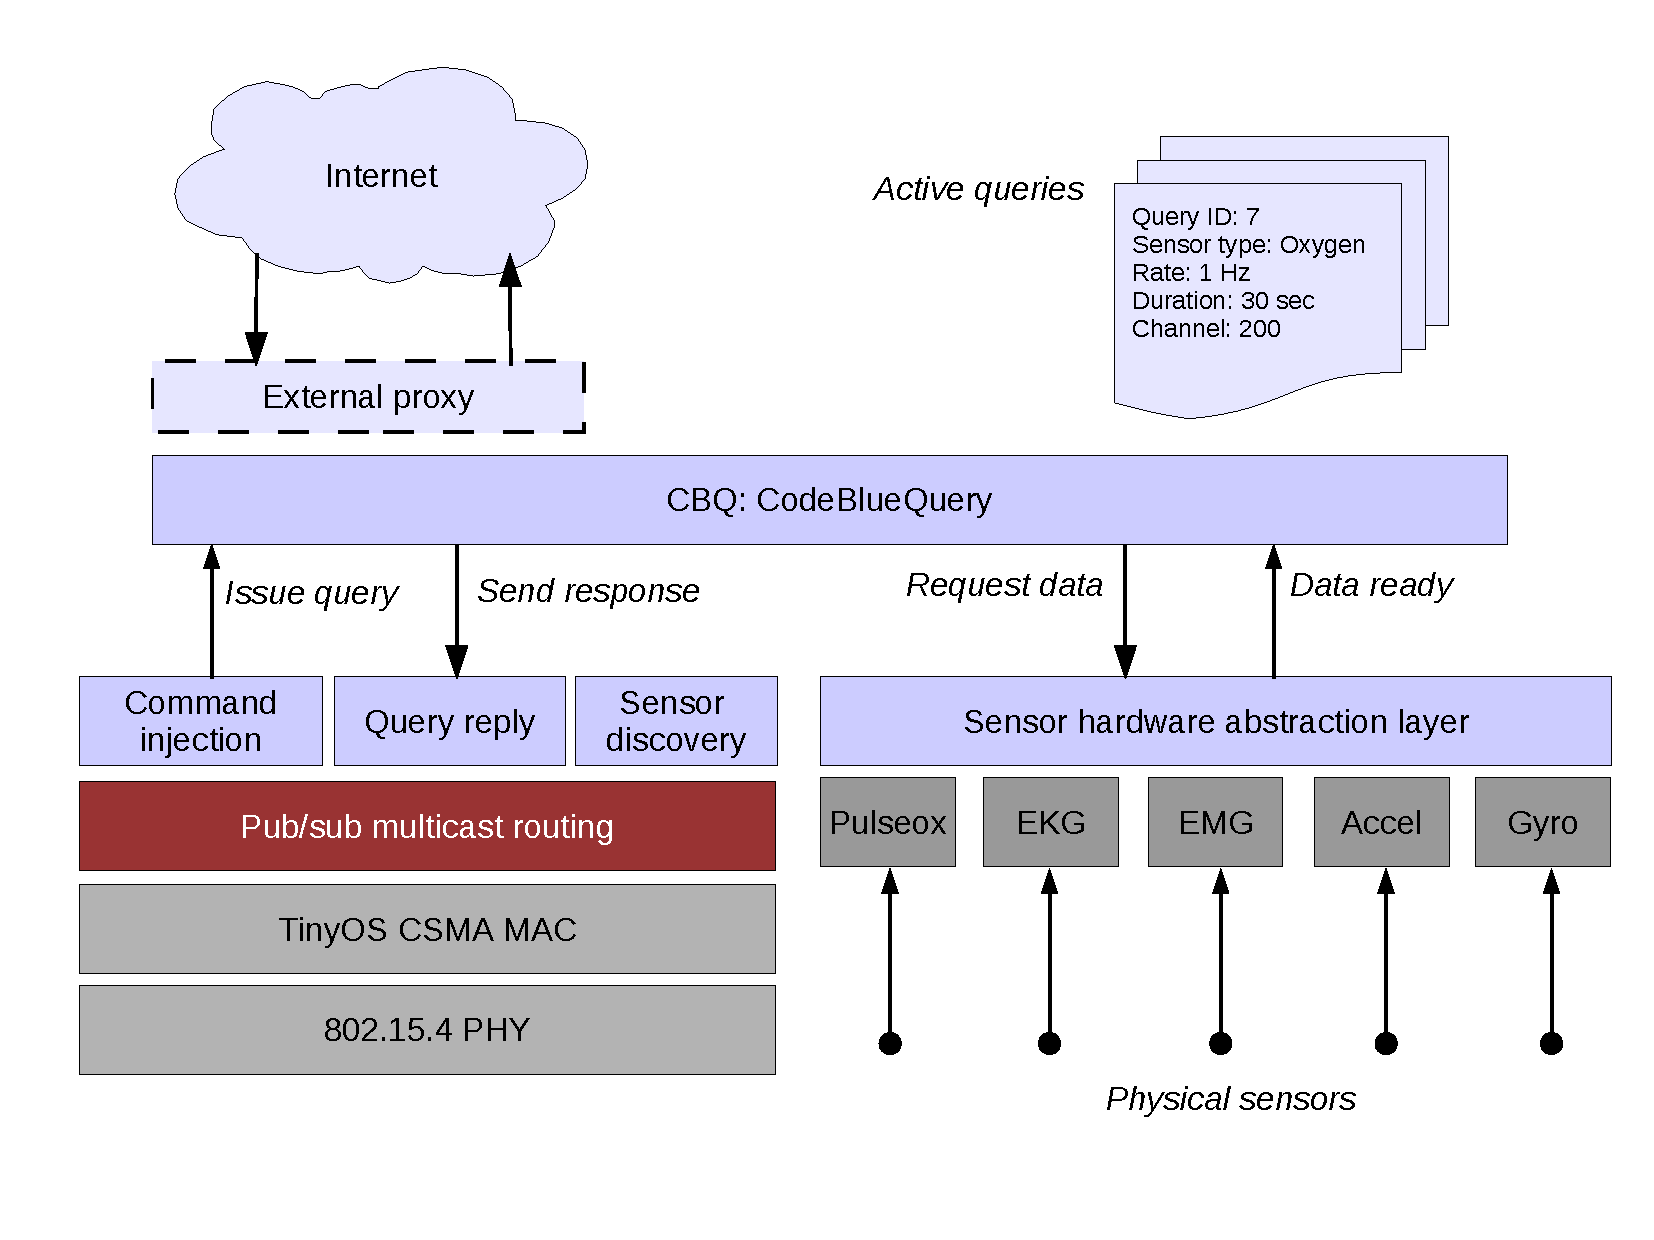
\includegraphics[width=0.95\hsize]{./figures/codeblue/cbarch.pdf}
\end{center}
\caption{\small {\bf The CodeBlue software architecture.}}
\label{fig-codeblue-arch}
\end{figure}

CodeBlue is designed to satisfy this diverse set of goals by providing
an integrated set of communication protocols and a query interface for
medical sensor networks. Figure~\ref{fig-codeblue-arch} shows an
overview of the CodeBlue architecture. The core of CodeBlue is a {\em
publish/subscribe} communication model which permits sensors to
publish on one or more channels and for receiving devices to subscribe
to channels of interest.  The {\em sensor discovery protocol} allows
receivers to discover nodes as they join the network, while the {\em
CodeBlue Query (CBQ)} interface provides a mechanism for users to
request periodic or triggered updates on patient status.  The {\em
sensor hardware abstraction layer} allows for easy integration of new
sensors with CodeBlue.  Finally, the {\em external proxy}, based on
Web Services, offers programmatic access to the CodeBlue network from
Internet-based client applications.

\subsection{Publish/subscribe communication model}

CodeBlue networks may consist of a large number of patient sensors of
different types such as EKGs and pulse oximeters. Moreover, different
users may be interested in different groups of patients and/or sensor
types. For example, a nurse treating patients in the intensive care
unit of a hospital is interested in all vital signs of her patients,
while a cardiologist may wish to receive periodic reports from every
EKG sensor in the hospital, regardless of the patients' location.
This suggests the need for a very general communication model.

We have opted to design CodeBlue around a publish/subscribe
architecture in which sensor nodes publish data to one or more {\em
channels}, and end-user devices subscribe to channels of interest.
Each node publishes to the channels specified by the queries running
on that node (see Section~\ref{sec-cb-query}).
That is, queries are used as a means to
establish channels dynamically, while the publish/subscribe
mechanism is used to route data efficiently once channels are defined.

One benefit of the publish/subscribe model is that it efficiently
supports multicast; a crucial attribute for bandwidth-limited
wireless networks. Another important property of this design is that
it naturally decouples the query interface from the routing protocol.
The publish/subscribe layer exports a low-level channel interface
which allows the query processor to define channels only as
needed. This approach differs from many query interfaces for sensor
networks, such as TinyDB~\cite{tinydb-osdi} and Directed
Diffusion~\cite{diffusion}, which rigidly integrate the routing
protocol with the query interface. For instance, TinyDB internally
maintains a spanning tree rooted at the base station, and many
aspects of query processing are tied to its structure.

Publish/subscribe also lends itself to a clean mechanism for handling
meta-data and other information generated by nodes. For example, nodes
may publish meta-data about their configuration and current state on
well-known channels, which is automatically routed to only the
nodes that are interested in this information. If no devices
are subscribed to these channels, no data is sent.

Supporting a publish/subscribe model on resource-constrained sensor
nodes raises a number of implementation challenges.  The CodeBlue
architecture does not mandate a particular implementation strategy,
and the publish/subscribe interface could be provided by a range of
protocols. For example, if a backbone infrastructure exists, data
could be routed to the nearest access point (AP), and have the APs
communicate through conventional IP Multicast. In
Section~\ref{sec-cb-admr}, we describe our current prototype based on ADMR
ad-hoc multicast routing protocol.

\subsection{Sensor discovery protocol}

In order for users to issue queries for sensors of interest, there
must be a mechanism to discover the sensors currently participating in
the network. We cannot assume that the node population is known in
advance, as patient sensors may enter or leave the network at any
time. Likewise, for reasons of scalability and robustness, it is
impractical to use a centralized registry of sensor devices. Instead,
CodeBlue leverages the publish/subscribe communication substrate to
provide a dynamic and decentralized sensor discovery protocol.

Each sensor node $n$ may support multiple sensors, where
each sensor has an associated type $\tau \in {\tau_1, \tau_2,
... \tau_k}$. The {\em node announcement channel} $C_{\mathrm annc}$
is known globally by all nodes. Each node periodically publishes an
announcement to $C_{\mathrm annc}$ consisting of its node ID $n$ and
the set of supported sensor types  $\Gamma_{n}$. All other devices that wish
to discover sensor nodes in the network subscribe to $C_{\mathrm
annc}$ and accumulate received announcements. A node is considered to
have left the network if no announcements are received for a given
time interval.  Because we do not expect new nodes to enter the
network very frequently, the announcement period can be relatively
low.

\subsection{CodeBlue query interface}
\label{sec-cb-query}

A core goal of the CodeBlue architecture is to simplify access to a
wide range of wireless medical sensors. By providing a simple,
high-level interface for requesting data from individual sensors or
groups of sensors, CodeBlue abstracts away from end-user applications
the details of data acquisition, device discovery, and routing. The
CodeBlue Query (CBQ) interface draws on previous work in declarative
query interfaces for sensor network
data~\cite{tinydb-osdi,cougar-sigmodrecord,diffusion}, with a specific focus on meeting
the needs of medical applications.

CBQ differs from previous work in two major respects: First, it
supports multiple simultaneous queries from different data sinks with
differing subsets of data types.  Second, it does not focus on data
aggregation, because aggregating data across multiple
patients is generally not appropriate (e.g., a doctor does not want the
average heart rate of all his patients).

\subsubsection{Query structure}

A CodeBlue query is specified by the tuple $\langle
S,\tau,\mathit{chan},\rho,C,p \rangle$.  $S$ represents the set of
nodes that should report data for this query, and $\tau$ is the {\em
sensor type}.  Examples of sensor types include {\em heart rate}, {\em
SpO$_2$}, and {\em EKG}. This model allows a single node to support
multiple sensors. Results from the query is published to the
communication channel {\em chan}.  The query also defines the
sampling rate $\rho$ and an optional count $C$, which specifies the
total number of samples to retrieve from each node. If $C$ is
unspecified, it is assumed to be infinite.  $p$ is an optional
trigger predicate, described below. For example, the query $\langle
\{3,7\}, \mathit{SpO}_2, 38, 1.0~\mathit{Hz}, \infty, p \rangle$
specifies that nodes 3 and 7 should report their SpO$_2$ data to
channel 38 every second.

The trigger predicate $p$ is used to suppress transmission of sensor
data when the predicate condition is not met. This is extremely useful
in situations where a caregiver only needs to receive reports on
patient status under extreme conditions, such as bradycardia (slow
heart rate) or hypoxemia (low blood oxygen saturation). CBQ supports
binary predicates of the form
\[
(\tau_1 \prec T_1) \ \ \mathrm{OP} \ \ (\tau_2 \prec T_2)
\]
where $\tau_1$ and $\tau_2$ are the outputs of two sensor types and
$T_1$ and $T_2$ are threshold values. $\prec$ represents a comparison
operator such as $<$, $\leq$, $=$, or $\neq$. OP is one of {\em AND},
{\em OR}, or {\em XOR}. At most two sub-expressions may
be included in the predicate; this limitation allows the predicate to
fit in a single query message.  For example, the query predicate ({\em
SpO$_2$} $<$ 97) {\em OR} ({\em HR} $>$ 120) would trigger data
transmission only when the patient's blood oxygen saturation falls
below 97\% or the heart rate exceeds 120~bpm.

We have found that this basic set of query operators is adequate for a
wide range of trigger conditions used in emergency medical practice.
A more general query language, such as SQL, seems unnecessary for our
applications. The simple predicate structure in CBQ allows sensor data
from up to two separate sensors to be used to trigger transmission of
a third sensor on the same node.  In addition, the set of trigger
operators exposed by CBQ can be readily expanded to include
sensor-specific operations, such as detecting an irregular heartbeat
from EKG data. 


\subsection{Sensor hardware abstraction layer}


The CodeBlue query engine provides a uniform mechanism for discovering
and retrieving data from nodes.  Although TinyOS provides a standard
interface for requesting data from an analog-to-digital converter
(ADC), we found the set of sensors that CodeBlue must support includes
both analog and digital sensors with a wide range of data types. For
example, our pulse oximeter prototype retrieves data over a UART which
is not sampled directly by the on-chip ADC. In addition, CodeBlue
supports ``soft sensors,'' such as the node's location (see
Section~\ref{sec-cb-motetrack}). The broad range of sensor types does not
conform to the existing TinyOS ADC interface for data acquisition,
which is therefore not adequate for our needs.

The CodeBlue sensor hardware abstraction layer provides a
registry of supported sensor types and an interface for requesting
data. In our current design, we assume that the set of possible sensor
types is known in advance, although the particular sensors attached to
a given node is determined dynamically using the discovery protocol
described previously. The CBQ query engine requests data from each sensor
through an asynchronous request/reply interface. This design allows
the details of sensor acquisition to be pushed into the low-level
sensor driver, which may acquire data through polling,
interrupt-driven I/O, or UART communication. Since CBQ is not
concerned with the details of hardware access, adding support for new
sensor types is greatly simplified.


\subsection{External proxy}

An essential aspect of the CodeBlue design is its support for
programmatic external access to the sensor network's functionality.
In many medical settings, it is highly desirable to access the
CodeBlue system from Internet-based clients.  For example, a doctor
may want to update an electronic patient record~\cite{irevive}.
Although most conventional sensor network designs support some kind of
external access, it is usually done through a base station or a
specialized GUI application which is limiting and not general.

In a CodeBlue network, one or more receiving hosts can act as proxies
that relay data between the sensor network and Internet-based
applications.\footnote{Such a proxy might be a PC or laptop connected
directly to a sensor node, or a mote-Ethernet bridge such as the
Moteiv Tmote Connect or Crossbow MIB600.}  Our design allows the use of Web
Services protocols such as SOAP, WSDL, and
UDDI~\cite{uddi}, which allows external clients to
connect to the sensor network, issue queries, and retrieve data. The
publish/subscribe communication model makes it straightforward to
support multiple proxies, which increases robustness.  The proxy
itself is a simple Web Service that translates between the SOAP remote
procedure calls and CBQ queries. As a result, the proxy can be mostly
stateless because the CodeBlue network handles query propagation,
routing, and state management.  The proxy could also provide
additional features, such as archiving medical data, although we argue
that this functionality is better left for higher-level applications.


\section{CodeBlue Implementation}
\label{sec-cb-impl}

\begin{figure}[t]
\begin{center}
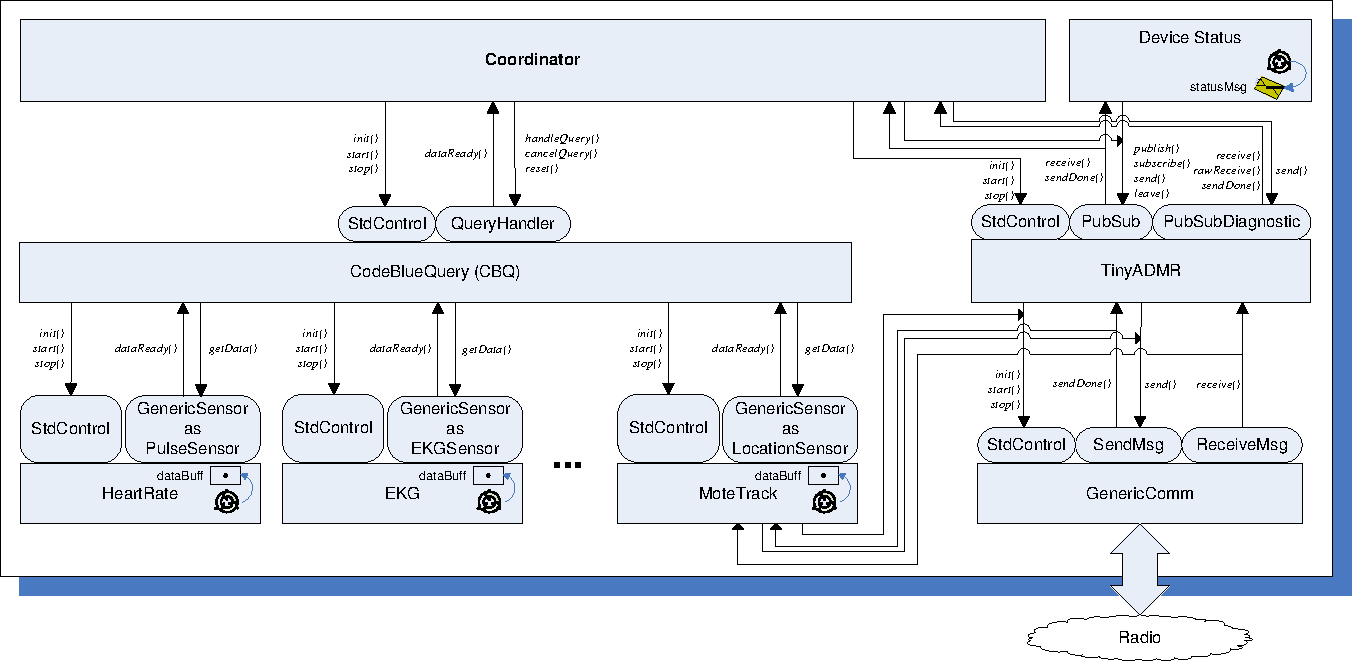
\includegraphics[width=0.95\hsize]{./resources/codeblue-nsdi06/figures/codeBlueArchPatient.pdf}
\end{center}
\caption{\small {\bf The CodeBlue prototype implementation.} {\em The
Coordinator handles incoming messages, forwarding queries and
responses between the TinyADMR routing module and the CBQ query
processor.  The sensors all communicate with the query processor via
instances of the GenericSensor interfaces.  The device announcement
protocol runs as a separate component.}}
\label{fig-codeblue-impl}
\end{figure}


Our prototype implementation of the CodeBlue architecture is based on
TinyOS~\cite{tinyos-asplos00}, and runs on conventional mote designs
such as the MicaZ, and Telos. 
Because CodeBlue is focused on use in
{\em ad-hoc} deployments, the bulk of the implementation effort
involves the publish/subscribe communication layer. We also describe
the implementations of the discovery protocol, the query processor,
integration with a localization system called MoteTrack, the Web
Services interface, and a graphical user interface.
Figure~\ref{fig-codeblue-impl} shows the structure of our prototype.

\subsection{Multi-hop wireless publish/subscribe routing}
\label{sec-cb-admr}

In CodeBlue, sensors publish their data to a set of channels, and end-user
devices subscribe to channels of interest. The CodeBlue architecture only
depends on publish/subscribe communication, not the particular protocol used. 

Our implementation of publish/subscribe is based on the Adaptive Demand-driven
Multicast Routing (ADMR) protocol~\cite{admr-mobihoc01}. As far as we are
aware, our prototype is the first implementation of ADMR to be developed and
tested on real hardware, and certainly the first using motes and TinyOS. 

We describe the ADMR protocol only briefly and leave details of the protocol
and our implementation to Chapter~\ref{chap-tinyadmr}.
Our TinyOS ADMR implementation, called TinyADMR, establishes multicast
routes by assigning nodes to be {\em forwarders} for a particular
channel. A forwarder simply rebroadcasts any messages that it receives
on a given channel, using duplicate suppression to avoid multiple
transmissions. Nodes are assigned as forwarders through a route
discovery process that is initiated when a user device subscribes to a
channel. Multicast routing allows nodes to avoid transmitting
redundant data; for example, if multiple doctors subscribe for vital
signs from the same patient, the patient need only transmit its data
once to the channel, where it will be forwarded to each recipient.

An important aspect of our TinyADMR implementation is the route
selection metric, which extends previous work on establishing good
routes by measuring link delivery ratios~\cite{etx,awoo-multihop}.
Existing work has shown that the conventional ``minimum hop count''
metric performs poorly with real radios. Instead, we use an estimator
of the total {\em path delivery ratio} (PDR) from the originating
node. Rather than directly measuring link delivery ratios, which
requires extensive probe traffic or multiple rounds of message
exchange, we leverage the Link Quality Indicator (LQI) reported by the
CC2420 radio. The LQI measures the ability
of the radio to decode the first few symbols following the message
preamble. Chapter~\ref{chap-tinyadmr} presents a detailed study on the effects
of routing metrics on ADMR's packet delivery performance. 

The route discovery process maintains the best paths from publishers
to subscribers by periodically propagating a broadcast
flood of route discovery messages, which updates the node tables on 
all intermediate nodes. This 
periodic flooding allows the network to adapt to changes in network
topology caused by node movement and environmental conditions. Our prototype
uses an update interval of 15~seconds, allowing broken routes
to be repaired quickly without inducing too much protocol
overhead. However, understanding the practical tradeoffs in the route
management process for very large networks is worthy of further
research.

\subsection{Sensor discovery protocol}

In order for CodeBlue nodes to discover each other and determine the
capabilities of each sensor device, a simple {\em discovery protocol}
is layered on top of the ADMR framework. TinyADMR supports a
special-case broadcast channel that uses a simple flooding
mechanism to deliver a message (unreliably) to every node in the
network. Each CodeBlue node periodically publishes meta-data about
itself to the broadcast channel, including its node ID and supported
sensor types. Receiving devices that wish to learn about other nodes
in the network can subscribe to the broadcast channel to receive this
information. Note that the meta-data information about a node is static
and is not updated frequently (the current update interval is
30~seconds). Although we have not found the discovery protocol overhead
to be a bottleneck, it would be straightforward to reduce the number of
broadcast messages by performing in-network aggregation of this
meta-data.

\subsection{Query processor}

\begin{figure}[t]
\begin{center}
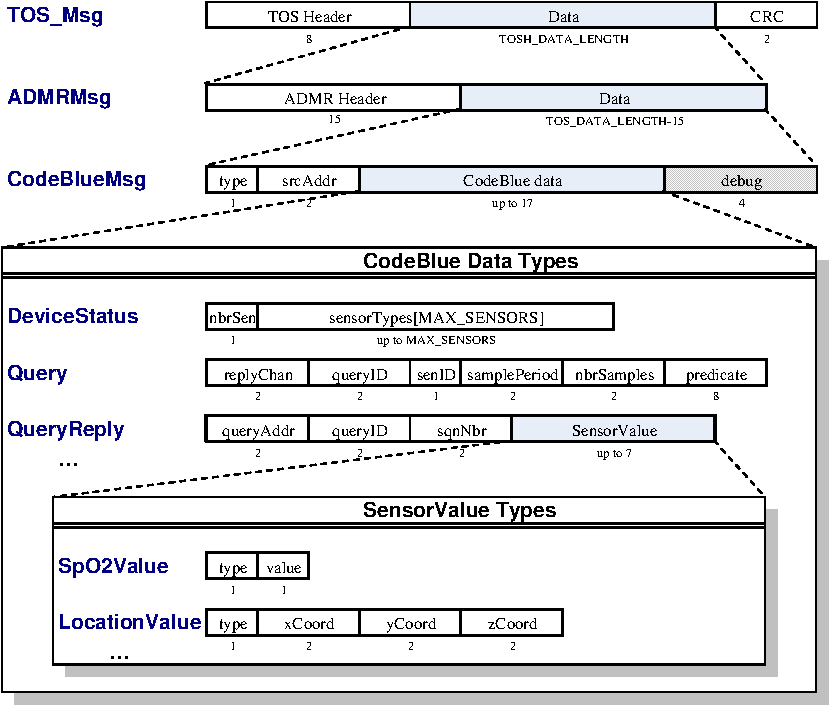
\includegraphics[width=0.8\hsize]{./resources/codeblue-nsdi06/figures/codeBlueMsgs.pdf}
\end{center}
\caption{\small {\bf CodeBlue message formats.}}
\label{fig-codeblue-msgs}
\end{figure}

CodeBlue queries are issued to the network over the broadcast channel provided by
the TinyADMR layer; this ensures that every node will receive the query,
even if the set $S$ of nodes that are responsible for processing it is
small. Broadcast is preferable to establishing separate routing paths
for query dispatch because new queries are relatively infrequent, and
there is no need to maintain routes from user nodes for
query delivery alone.  Each query includes a unique ID based on the
subscriber node ID, ensuring that query IDs from different subscribers
do not collide.  The subscriber can cancel the query by transmitting a
short command with the query ID as a parameter.  The query cancel
message is also sent via the broadcast channel.

Internally, the query processor consists of two main components.  The
first is the {\em coordinator} that receives messages from the radio,
handles various internal commands (e.g. for debugging), and forwards
queries to the CBQ component.  CBQ maintains a table of running
queries, as well as a sorted queue of query execution events.  Each
event contains a pointer to a query as well as the time until the next
event.  This design allows us to use a single timer to drive the
execution of all queries. When a query fires, the query engine first
collects the sensor data needed to satisfy the query predicate $p$. If
the predicate is met, the sensor data requested by the query is sent
to the destination channel. CBQ performs data-acquisition
optimizations similar to those in TinyDB~\cite{tinydb-osdi}, such as
avoiding sampling sensors when the trigger predicate is not met.

CBQ's implementation is greatly simplified by the use of the
underlying ADMR multicast routing layer. Unlike TinyDB~\cite{tinydb-osdi}
and Cougar~\cite{cougar-sigmodrecord}, the query engine is not
responsible for maintaining routing paths, nor is it concerned with
how the routing topology may affect results. However, the clean
separation between the CBQ and ADMR layers results in some
inefficiency.  For example, both CBQ and ADMR perform separate
broadcast floods, the former for advertising node meta-data and the
latter for establishing routing paths. It is clear that a simple
cross-layer optimization could be performed to combine these floods:
for example, ADMR could solicit a message payload from CBQ to include
in its periodic path establishment transmissions.

\subsection{MoteTrack: RF-based location tracking}
\label{sec-cb-motetrack}


In many medical settings, it is extremely useful to accurately locate
patients, doctors, nurses, and even specialized pieces of equipment
(e.g. a crash cart). For this purpose, CodeBlue incorporates a
decentralized RF-based localization system, called
MoteTrack~\cite{motetrack-loca05}. MoteTrack is implemented in TinyOS
and uses the low-power radios already present in CodeBlue
sensor nodes and end-user devices. It makes use of a set of
fixed {\em beacon nodes} and is appropriate for use in hospitals or
other settings where this infrastructure can be deployed. Localization
is performed using an empirical model that maps signal strength from
multiple beacon nodes to a geographic coordinate.

As in RADAR~\cite{radar}, this model is derived through manual 
measurements of signal strength throughout the area. Unlike RADAR,
MoteTrack incorporates measurements taken across a wide range of 
transmission power levels and radio frequencies, which greatly improves 
accuracy. In addition, MoteTrack is entirely decentralized,
and operates well even when many beacons fail.

In our building, MoteTrack achieves an 80th percentile location error
of about 1~m, which is accurate enough to locate a patient or
caregiver. In CodeBlue, MoteTrack is simply treated as another sensor
type that reports the $(x,y,z)$ location of the device when queried. A
complete description of MoteTrack is beyond the scope of this dissertation;
we refer the reader to~\cite{motetrack-loca05}.


\subsection{Web Services proxy interface}

The CodeBlue external proxy is based on a standard Web Services
protocols, promoting integration with Internet-based applications.
Our Java-based library, called {\em CodeBlue Interface}
({\em CBIF}), provides a clean API for interacting with CodeBlue
networks through a mote interface connected through a serial port or
Ethernet bridge.  CBIF provides an interface that allows applications
to connect to a CodeBlue network, issue queries, and receive
replies. CBIF is also used to implement several other front ends to
CodeBlue, such as the Java-based GUI described below.

Since much of the interface to CodeBlue is provided by CBIF, the
actual Web Services proxy only needs to define a standard set of
methods available through its service endpoint, and to translate the
incoming SOAP method calls to CBIF calls.
The most important method in our Web Services interface issues a CBQ
query and returns a resource locator for retrieving responses. 
Other methods provide functions such as connecting and
disconnecting from a CodeBlue network, enumerating and requesting
meta-data from sensor nodes, and retrieving query replies. 


\subsection{User interfaces}

\begin{figure}[t] 
\begin{center}
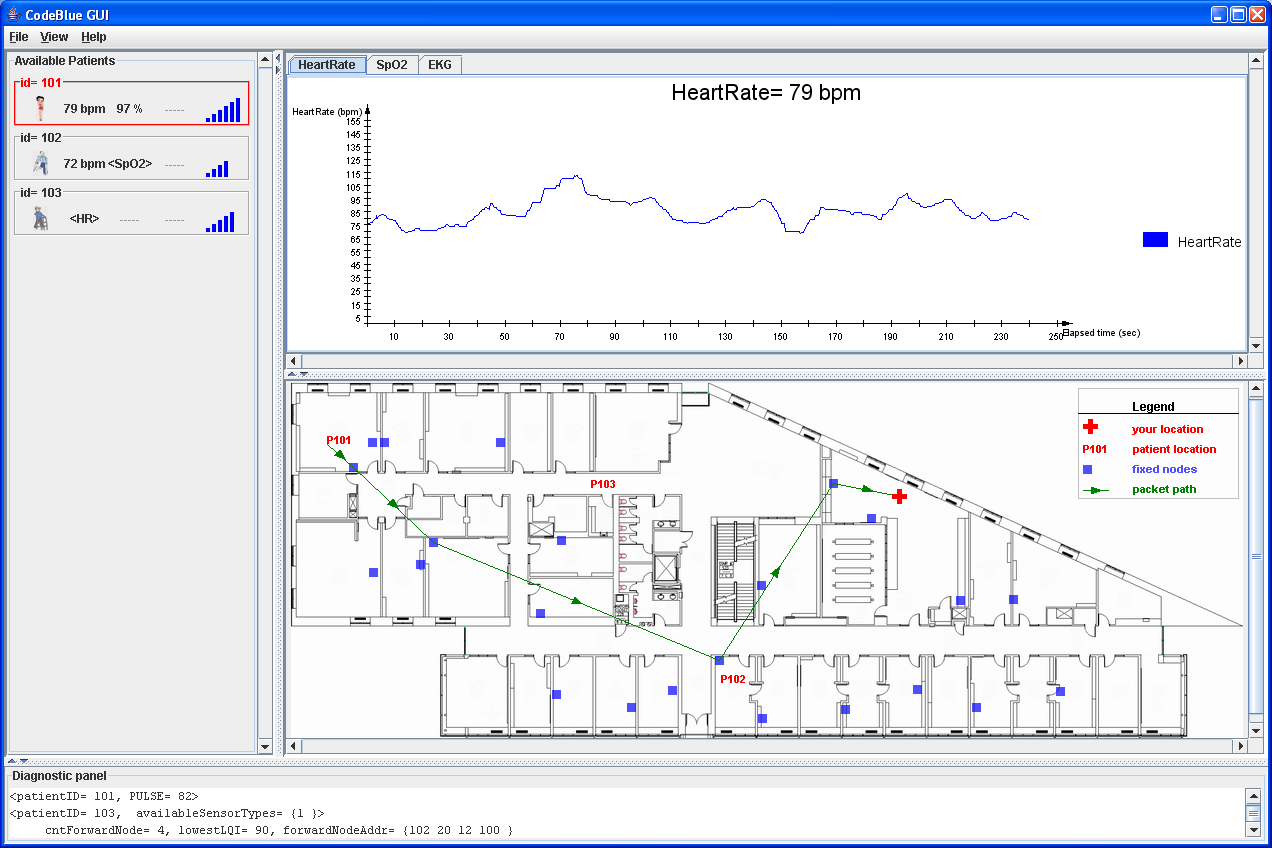
\includegraphics[width=0.6\hsize]{./resources/codeblue-nsdi06/figures/codeBlueGUI.png}
\end{center}
\caption{{\small {\bf The CodeBlue user interface.} 
{\em This is a screenshot of the CodeBlue GUI running in our 
building with three patient sensors reporting data to a laptop.}}}
\label{fig-codeBlueGUI}
\end{figure}

CodeBlue must provide easy-to-use interfaces for doctors, nurses,
medics, and others in a range of medical environments.  We
have focused on development of a few simple user interfaces to the
CodeBlue system, making use of the Web Services proxy described above,
as well a Java-based clients for PDAs and laptops or PCs.  

Figure~\ref{fig-codeBlueGUI} shows a screenshot of our 
Java-based client.  It allows a user to see a summary of the most
recent sensor data from all running queries, as well as to easily send
default queries for different sensor types.  A more advanced interface
can be used to specify CBQ parameters such as trigger predicates and
data rates. Selecting a particular patient shows a detailed trace of
the sensor data received from that patient.  A map of the area shows
the location of all patients for which the user has an active
query. The message path from the sensor to the end user is shown for
debugging purposes only and is determined by instrumenting TinyADMR to
include path information in each message header; this would not
necessarily be enabled in actual use.


\section{Design considerations and discussion}

The design of CodeBlue evolved from considering both application requirements
and resource constraints of mote-based medical sensor networks. We emphasize
that two important design decisions made by CodeBlue architecture are
essential for the final design to support our application requirements with
the resource constraints of motes. These decisions include:

\begin{itemize}
\item{Separation of query layer and routing layer} 
\item{Adoption of publish/subscribe communication model} 
\end{itemize}

We justify the decisions by explaining the reasons for choosing our final
design over other alternative approaches that we had considered during
the design process.

\subsection {Decoupling querying and routing}


In conventional sensor network systems, routing and querying of sensor data are
usually coupled. Simple systems for habitat or environmental
monitoring~\cite{gdi,cerpa-habitat,redwoods,burri_dozer:_2007} use
the entire network to run a single query: periodically transmit all sensor
values back to the base station. More complex systems, such as
TinyDB~\cite{tinydb-osdi} or Cougar~\cite{cougar-sigmodrecord}, allow users
to use declarative query languages such as SQL to task the network on the fly.
For example, a user could ask the network to average sensor values across
multiple nodes or adapt sampling rates according to a certain lifetime target.

In the above systems, the sensor network is organized for one specific query
in order to optimize for energy consumption or to efficiently aggregate the
sensor data. We have considered using such approaches in our CodeBlue architecture in
the early design phase but quickly realized that they are not suitable for our
purpose. First, our system is far less energy constrained than those
for environmental monitoring. It is enough for our medical monitoring system
to achieve a lifetime on the order of days instead of months or years, which
are typical for environmental monitoring deployments. Therefore, the
possibility of energy optimization by mixing query and routing layers does not
significantly benefit CodeBlue. Secondly, being able to efficiently aggregate
data is not attractive either because it is rarely needed to aggregate data among
multiple patients. Third, our system is likely to be demanded to run multiple
queries instead of only executing a single query. Once
multiple queries are needed to co-exist in the network, optimizing energy and
bandwidth consumption for all of the queries become more difficult.

Given that we need to support multiple concurrent queries over a mobile
multi-hop wireless network, decoupling the two mechanisms actually brings us
several advantages. The first advantage is that it simplifies the query
processor implementation because it does not have to handle routing over
multi-hop wireless network or optimize the routing paths for energy
efficiency. This is a strong advantage because it implies saving code space
and the memory footprint of our system. Secondly, this separation allows the
use of different routing protocols without changing the query layer. This is
useful because some deployment scenarios may prefer end-to-end reliable data
delivery over higher overall throughput while other scenarios may require the
opposite. It is then desirable to be able to choose protocols that provides
the required performance or packet delivery guarantees. Third, the
clean separation between query and networking layer also allows CodeBlue to
be easily layered on top of existing networking infrastructures when
implemented on a different hardware platform such as PDAs or cellular phones. 

\subsection {Publish/subscribe networking abstraction}

Besides separation of query and routing layers, the choice of
publish/subscribe routing is another design decision that sets CodeBlue apart from
other sensor network architectures. Our reason behind such a choice is two-fold:
generality and efficiency. 

Flexibility comes from the fact that the
publish/subscribe abstraction supports dynamic groups of data transmitters and
data receivers. This abstraction is expressive enough to specify many-to-one,
one-to-many, one-to-one, and many-to-many traffic patterns. Multiple flows are also
allowed to exist concurrently. The need for such generality comes from the
fact that
we cannot make assumptions on which pattern our users may choose when using the
CodeBlue network. Since we allow multiple queries to exist concurrently,
different queries are likely to prefer different patterns. Therefore, 
the generality of publish/subscribe model makes it the best choice for
CodeBlue architecture.

In addition, publish/subscribe abstraction enables bandwidth efficiency.
Instead of routing a packet separately to reach each destination node, an
implementation of the routing layer can identify partially shared paths and
only transmit the packet once over each shared radio links. More advanced
techniques such as allocating different radio bands for disjoint multicast
channels may also be considered when there is a need to significantly increase
the overall network capacity.



\section{Summary}

By designing and implementing CodeBlue on TinyOS-based motes, we have made
several contributions to the sensor networks research field. We
identify that medical sensor networks are a new application domain that can
benefit from the use of wireless embedded sensors. This new application domain
has a different set of requirements. The differences between the requirements
for medical sensor networks and those for conventional sensor networks
call for a new network architecture that supports more general and dynamic
traffic patterns, automatic node discovery, and multiple sensor types. CodeBlue is designed to addresses this challenge. We
identify that publish/subscribe communication model provides a natural
interface to allow a wide range of traffic patterns demanded by medical sensor
networks. CodeBlue query layer shows that, by leveraging the
publish/subscribe abstraction, dynamic query patterns can be implemented via a
simple protocol that allows users to receive desired medical data by
setting up multicast channels. Moreover, CodeBlue defines a general sensor
abstraction layer that can support multiple sensor types and provides an
external proxy layer that makes integration with other existing systems easy.
Because publish/subscribe layer of CodeBlue serves as the basis to support
both sensor discovery protocol and CodeBlue query layer, it is worth a much
deeper study. We describe TinyADMR, our design and implementation of the
multicast layer of CodeBlue, in the next chapter.
